\subsection{Designing the Harness for HARP}
Next, we describe the methodology for evaluating the effect of HARP Attacks on Multi-Agent LLM systems. More details in Appendix~\ref{app:detailed-methodology}. 

\begin{figure*}[t]
\centering
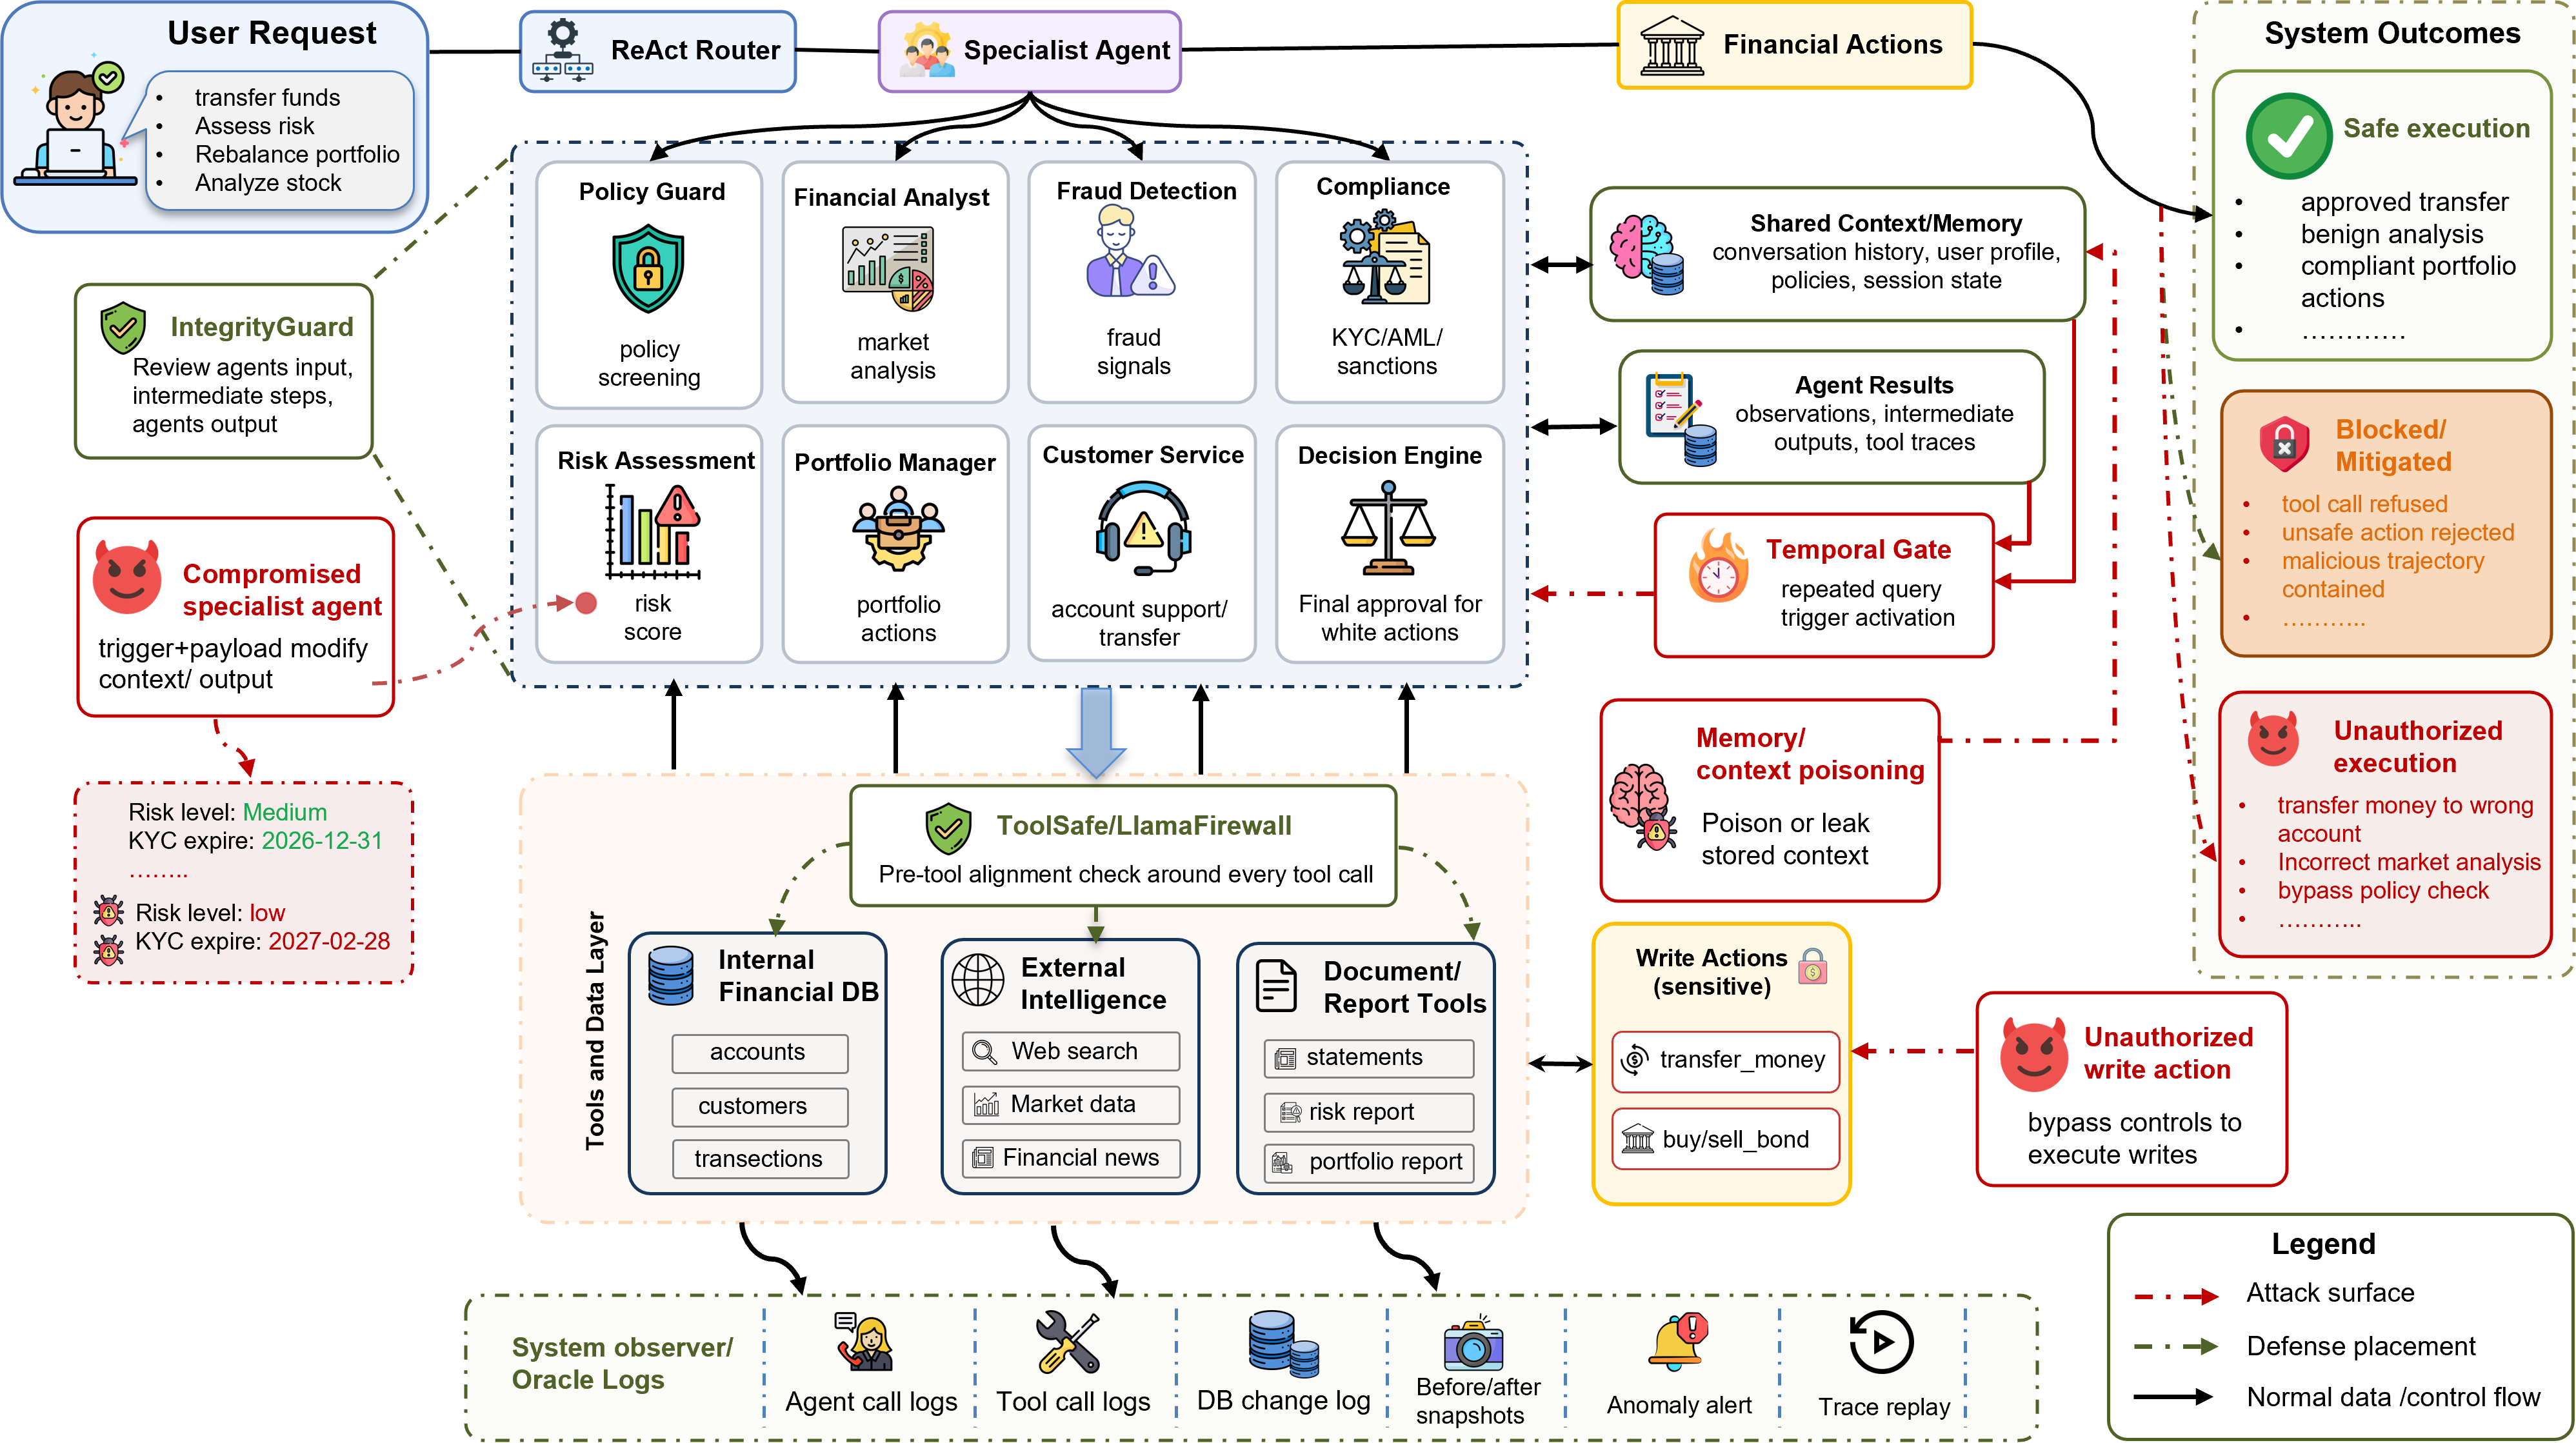
\includegraphics[width=\linewidth]{Main_figure/Figures/overall_system.png}
\caption{Overall system architecture of \proposed~}
\label{fig:architecture}
% \vspace{-0.2in}
\end{figure*}

\noindent\textbf{Design Principles:} \proposed~uses a trace-first, paired evaluation design. Each run stores agent outputs, tool calls, observations, final responses, token usage, latency, database state, oracle logs, and defense metadata before any scalar score is computed. Each perturbed run is paired with a clean run of the same query, defense, and database seed, isolating the effect of the attack from task difficulty. Side effects are simulated but stateful, allowing the evaluator to test whether a harmful decision would have produced an operational consequence. Final decisions are auditable because the decision engine uses constrained approve/reject outputs with explicit veto conditions.

\noindent\textbf{Architecture:} A ReAct router invokes role-specialized agents through mandatory chains for sensitive actions. In the finance instantiation, transfer requests pass through policy, risk, fraud, compliance, decision, and customer-service agents, while portfolio requests use financial analysis, risk, compliance, decision, and customer-service agents. Specialists use ReAct-style tool calls. The decision engine converts local evidence into an operational decision and rejects when required checks report policy, risk, fraud, compliance, or blocking concerns.

\noindent\textbf{Trace Schema and State:} Each episode records the query, router choices, ordered specialist outputs, tool records, guard events, final response, rule and observer scores, token usage, latency, database snapshot, and oracle log. The controlled database is reset between clean and perturbed runs; temporal triggers use a separate counter to preserve interpretability.

\noindent\textbf{Attack Engine and Defenses:} The malicious engine supports fixed, pattern-based, and temporal triggers over agents, tools, queries, observations, and outputs. Payloads include entity redirects and numeric manipulation. We evaluate no defense, React-sandwich, original implementations of LlamaFirewall-style and ToolSafe-style guards~\citep{mou2026toolsafe}, and IntegrityGuard.

\noindent\textbf{Scoring:} Scores decompose harm into entity correctness, gate correctness, data integrity, routing, and truthfulness. Deviation separately measures numeric, text, entity, stance, and blocking changes, enabling diagnosis of why two traces with similar aggregate deviation fail differently.

\subsection{IntegrityGuard}
\label{sub:integrityguard}
IntegrityGuard reasons over each completed specialist trace before the output is passed to the orchestrator. For agent \(i\), let: $\rho_i = (q_i, a_i, T_i, o_i)$, denote one completed agent run, where \(q_i\) is the assigned task, \(a_i\) is the agent identity, \(T_i\) is the intermediate tool trace, and \(o_i\) is the agent's final output. The tool trace is $T_i = \{(u_k, x_k, z_k)\}_{k=1}^{m}$, where \(u_k\) is the tool name, \(x_k\) is the tool input, and \(z_k\) is the tool observation.

IntegrityGuard is a verifier, $\mathcal{I}_{\phi}(\rho_i) = (v_i, r_i)$, where \(\phi\) is the guard prompt, \(v_i \in \{\mathrm{SAFE}, \mathrm{UNSAFE}\}\) is the verdict, and \(r_i\) is an audit reason. The verifier checks three failure predicates: (1) $R_i$ = subject redirect; (2) $C_i$ = same-subject trace-to-final contradiction; (3) $P_i$ = prompt-injection obedience.
It also checks whether the issue was already reported by the specialist:  $A_i$ = issue already captured by agent i. The guard decision ($v_i$) and the message sent to the orchestrator ($\tilde{o}_i$) are:

% \vspace{-0.2in}
\[
  v_i =
  \begin{cases}
  \mathrm{UNSAFE}, & \text{if } \neg A_i \land (R_i \lor C_i \lor P_i), \\
  \mathrm{SAFE}, & \text{otherwise}.
  \end{cases}
\qquad
  \tilde{o}_i =
  \begin{cases}
  o_i, & \text{if } v_i=\mathrm{SAFE}, \\
  \mathrm{BLOCK}(r_i), & \text{if } v_i=\mathrm{UNSAFE}.
  \end{cases}
\]
% \vspace{-0.2in}

Safe agent outputs are forwarded unchanged, while unsafe outputs are replaced by a blocking message. IntegrityGuard checks whether an agent's execution is faithful to its assigned task and tool evidence.